\def\homeworknumber{3}
\def\homeworkdate{25-10-2011}

\documentclass[11pt]{article}
\linespread{1}

\renewcommand{\thefootnote}{\fnsymbol{footnote}}

\usepackage{geometry} % see geometry.pdf on how to lay out the page. There's lots.
\usepackage[utf8]{inputenc}
\usepackage{array}
\usepackage{amsmath,amssymb,latexsym,epic,eepic,epsfig,graphics,psfrag}
\usepackage{amsfonts}
\usepackage{graphicx,float}

\usepackage[danish]{babel}

\usepackage[bottom]{footmisc}

\usepackage{fancyhdr}
\pagestyle{fancy}
\lhead{\small\textit{01246 Partial Differential Equations - Fall 2011 - Anders Hørsted (s082382)}}
\rhead{\thepage}
\chead{}
\lfoot{}\cfoot{}\rfoot{}

\usepackage{pstricks}
\usepackage{pst-node}
\usepackage{wrapfig}
\usepackage{caption}
\usepackage{multirow}
%\usepackage{fouriernc}
%\usepackage[charter]{mathdesign}
\usepackage{lmodern}
\usepackage[normalem]{ulem}
\geometry{a4paper} % or letter or a5paper or ... etc
% \geometry{landscape} % rotated page geometry

\usepackage{subfigure}
\usepackage{placeins}
\usepackage{url}
\usepackage{natbib}
\renewcommand\bibsection*{}
\bibliographystyle{plain}

\makeatletter
\renewcommand*\env@matrix[1][*\c@MaxMatrixCols c]{%
  \hskip -\arraycolsep
  \let\@ifnextchar\new@ifnextchar
  \array{#1}}
\makeatother

\newcommand\myimp{\quad\Leftrightarrow\quad}
\newcommand\half{\frac{1}{2}}
%\newcommand\myvec[1]{\mathbf{#1}}
\newcommand\myvec[1]{\boldsymbol{#1}}
\newcommand\vecx{\myvec{x}}
\newcommand\mymod[1]{\ (\text{mod }#1)}
\newcommand\myreal{\mathbb{R}}
\newcommand\mynatural{\mathbb{N}}
\newcommand\myinteger{\mathbb{Z}}
\newcommand\mycomplex{\mathbb{C}}
\newcommand\myint{\text{int}}
\newcommand\norm[1]{||\,#1\,||}
\newcommand\bignorm[1]{\big|\big|\,#1\,\big|\big|}
\newcommand\seq[1]{\big\{#1\big\}}
\newcommand\smallseq[1]{\{#1\}}
\newcommand\smallseqtoinf[1]{\smallseq{#1}_{k=1}^\infty}
\newcommand\lonew{\ell^1_w}
\newcommand\lone{\ell^1}
\newcommand\ltwo{\ell^2(\mynatural)}
\newcommand\ip[2]{\langle#1,#2\rangle}
\newcommand\hilbert[1]{\mathcal{#1}}
\newcommand\uinf{u_{\infty}}
\newcommand\erf{\text{erf\,}}
\newcommand\infint{\int_{\infty}^{\infty}}
\newcommand\celsius{$^\circ$C}
\newcommand\comsol{Comsol}
\newcommand\fourier{\mathcal{F}}

\usepackage{tabulary}
\newcolumntype{y}{>{\centering\arraybackslash}R}

\setlength{\unitlength}{2mm}
\usepackage{tikz}

\title{Homework \homeworknumber}
\author{01246 Partial differential equations -- \homeworkdate -- Anders Hørsted (s082382)}
%\author{}
\date{} % delete this line to display the current date


\begin{document}
    \maketitle

    \section*{Exercise 1}
    The annulus $A$ is given in polar coordinates by $r\in(1,2), \theta\in(0,2\pi)$. A PDE problem is defined by
    \begin{gather}
        \Delta u = 0 \text{ in }A \\
        u(1,\theta) = 0,\quad \frac{\partial u}{\partial r}(2,\theta) = 1 - 2\cos(\theta),\quad \theta\in(0,2\pi)
    \end{gather}
    The solution to this PDE problem is now found. The solution formula 6.4.7 in the textbook can be used for this problem. Using the first boundary condition we get that
    \begin{align*}
        u(1,\theta) &= \frac{1}{2}(C_0 + D_0\log(1)) + \sum_{n=1}^\infty (C_n+D_n)\cos(n\theta) + (A_n+B_n)\sin(n\theta) \\
        &= 0
    \end{align*}
    from which we conclude that $C_0=0, C_n=-D_n, A_n=-B_n$. Since
    \begin{align*}
        u_r(r, \theta) = \frac{1}{2}D_0r^{-1} + \sum_{n=1}^\infty (C_n n r^{n-1} - D_n n r^{-n-1})\cos(n\theta) + (A_n n r^{n-1} - B_n n r^{-n-1})\sin(n\theta)
    \end{align*}
    we get from the second boundary condition that
    \begin{align*}
        u_r(2, \theta) &= \frac{1}{4}D_0 + \sum_{n=1}^\infty (C_n n 2^{n-1} - D_n n 2^{-n-1})\cos(n\theta) + (A_n n 2^{n-1} - B_n n 2^{-n-1})\sin(n\theta) \\
        &= \frac{1}{4}D_0 + \sum_{n=1}^\infty (2^{n-1} + 2^{-n-1})C_n n \cos(n\theta) + (2^{n-1} + 2^{-n-1})A_n n \sin(n\theta) \\
        &= 1 - 2\cos(\theta)
    \end{align*}
    from which we get that $D_0=4, C_1=-\frac{8}{5}, D_1=\frac{8}{5}$ and all other coefficients should be 0. The solution is therefore given by
    \begin{equation*}
        u(r, \theta) = 2\log{(r)} + (\frac{8}{5}r^{-1} - \frac{8}{5}r)\cos(\theta)
    \end{equation*}
    The solution is plotted and is shown in figure~\ref{fig:q1-plot}. From the figure it is seen that the solution takes on its minima at $(2,0)$ and maxima at $(2,\pi)$. Both point are on the boundary as expected from the maximum principle.
    \begin{figure}
        \centering
        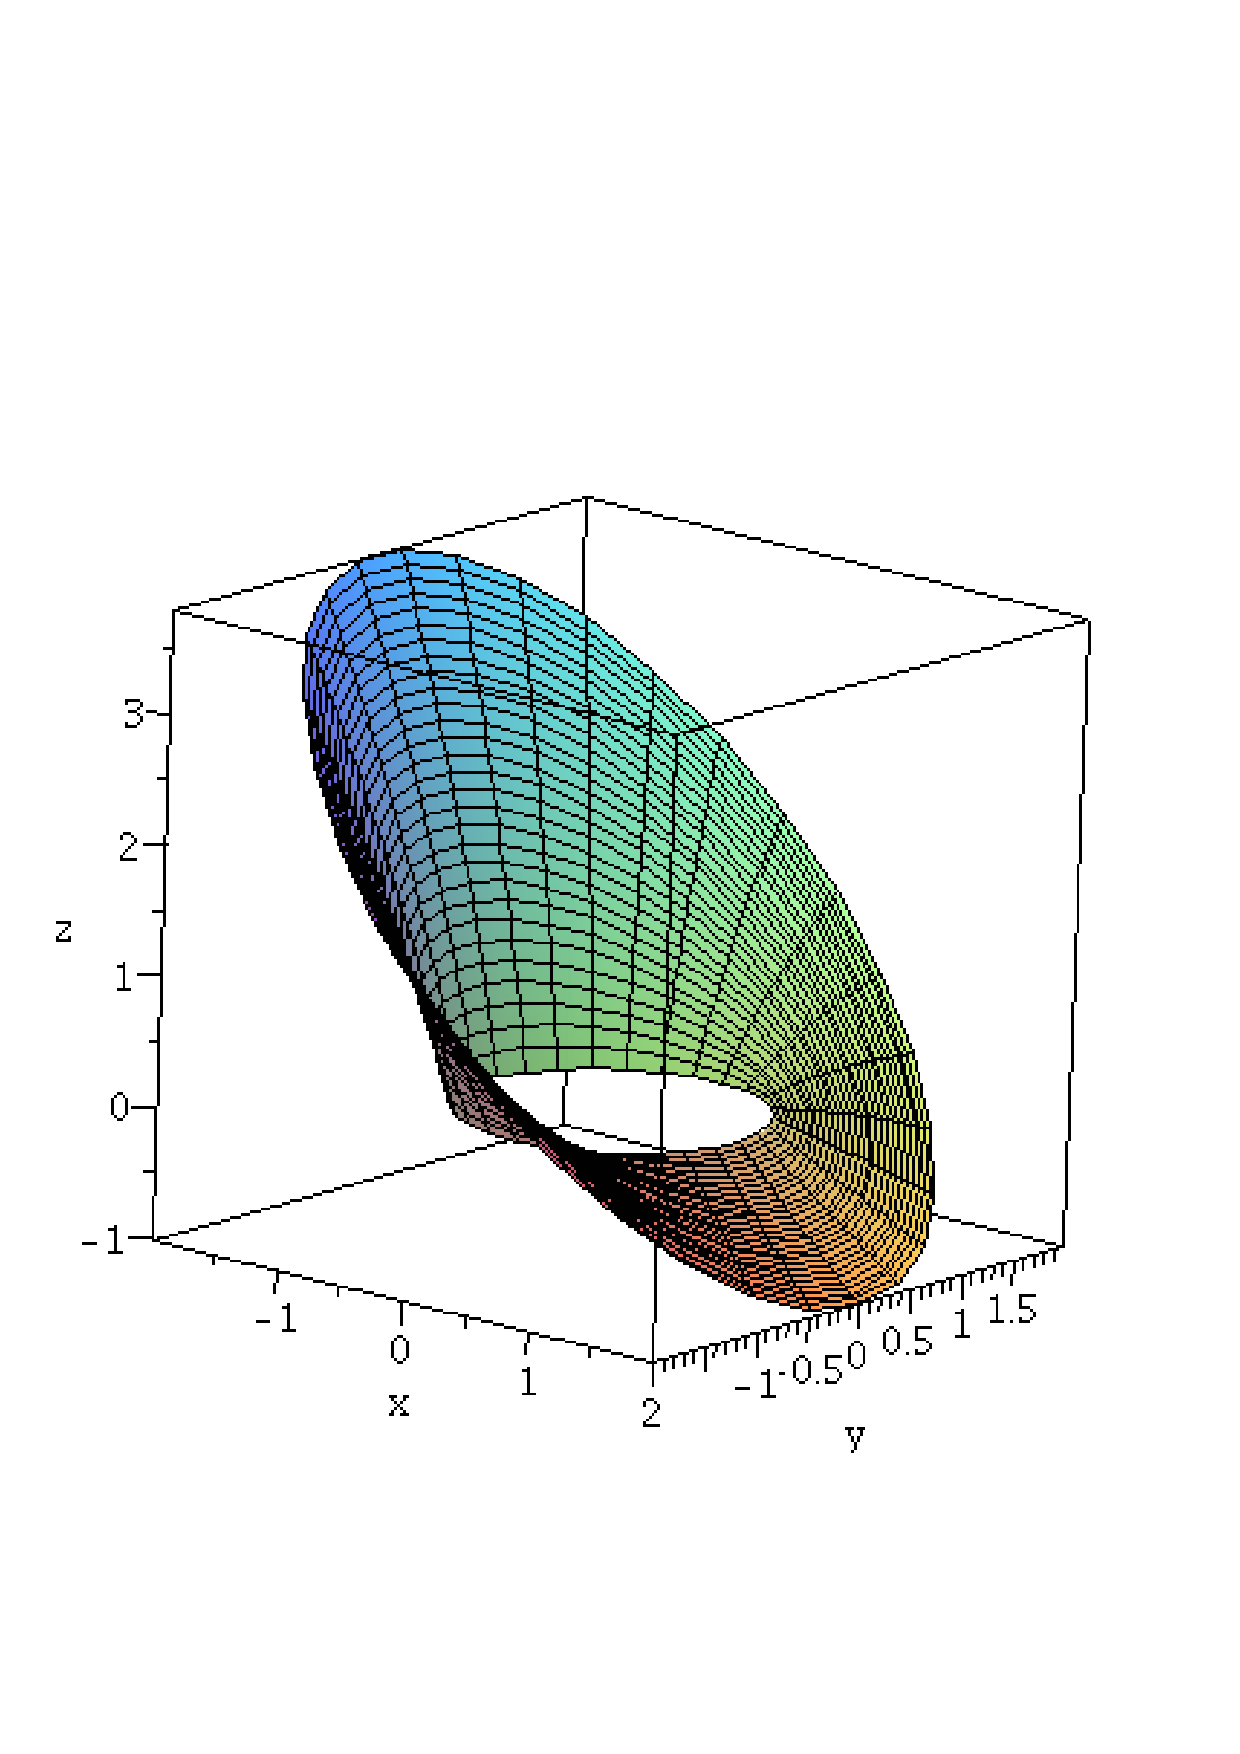
\includegraphics[width=90mm]{q1-plot.png}
        \caption{Plot of solution for exercise 1}
        \label{fig:q1-plot}
    \end{figure}

    \section*{Exercise 2}
    Using the reflection method the Green's function $G$ for the Laplace Equation in the half plane $H=\{(x,y)\,|\,x\in\myreal,\:y>0\}$ is found. Based on the derivation of the Green's function in the half space in the textbook combined with the representation formula in two dimensions (eq. 7.2.5) a good guess for $G$ is
    \begin{equation*}
        G(\vecx, \vecx_0) = \frac{1}{2\pi}(\log|\vecx-\vecx_0| - \log|\vecx-\vecx_0^*|)
    \end{equation*}
    that in coordinates becomes
    \begin{equation}\label{eq:green-coord}
        G(\vecx, \vecx_0) = \frac{1}{2\pi}(\log((x-x_0)^2 + (y-y_0)^2)^{1/2} - \log((x-x_0)^2 + (y+y_0)^2)^{1/2})
    \end{equation}
    By exactly the same arguments as in the textbook p. 191-192 it can be ``proved'' that $G$ is the Green's function for $D$ at $\vecx_0$. \par
    We now use $G$ to solve the Dirichlet problem
    \begin{gather*}
        \Delta u = 0 \text{ in } H, \\
        h(x) = u(x, 0) = \begin{cases}
            1, & x\in(-1,1) \\
            0, & \text{elsewhere}
        \end{cases}
    \end{gather*}
    To solve the problem, $\frac{\partial G}{\partial n}=-\frac{\partial G}{\partial y}|_{y=0}$ must be determined.
    \begin{align*}
        -\frac{\partial G}{\partial y} &= \frac{1}{2\pi}\left(\frac{y+y_0}{|\vecx-\vecx_0^*|^2} - \frac{y-y_0}{|\vecx-\vecx_0|^2}\right)
        \intertext{\textit{that at the boundary ($y=0$) becomes}}
        &= \frac{y_0}{\pi((x-x_0)^2 + y_0^2)}
    \end{align*}
    Using theorem 7.3.1 the solution of the Dirichlet problem is then given as
    \begin{align*}
        u(x_0, y_0) &= \int_\infty^\infty h(x)\frac{y_0}{\pi((x-x_0)^2 + y_0^2)}\,dx \\
        &= \frac{1}{\pi}\int_{-1}^{1} \frac{y_0}{((x-x_0)^2 + y_0^2)}\,dx \\
        &= \frac{1}{\pi}\left(\arctan\left(\frac{x_0+1}{y_0}\right) + \arctan\left(\frac{1-x_0}{y_0}\right)\right)
    \end{align*}
    The solution is plotted and shown in figure~\ref{fig:q2-plot}. It is again found that both the minimum and maximum is obtained at the boundary.
    \begin{figure}[ht]
        \centering
        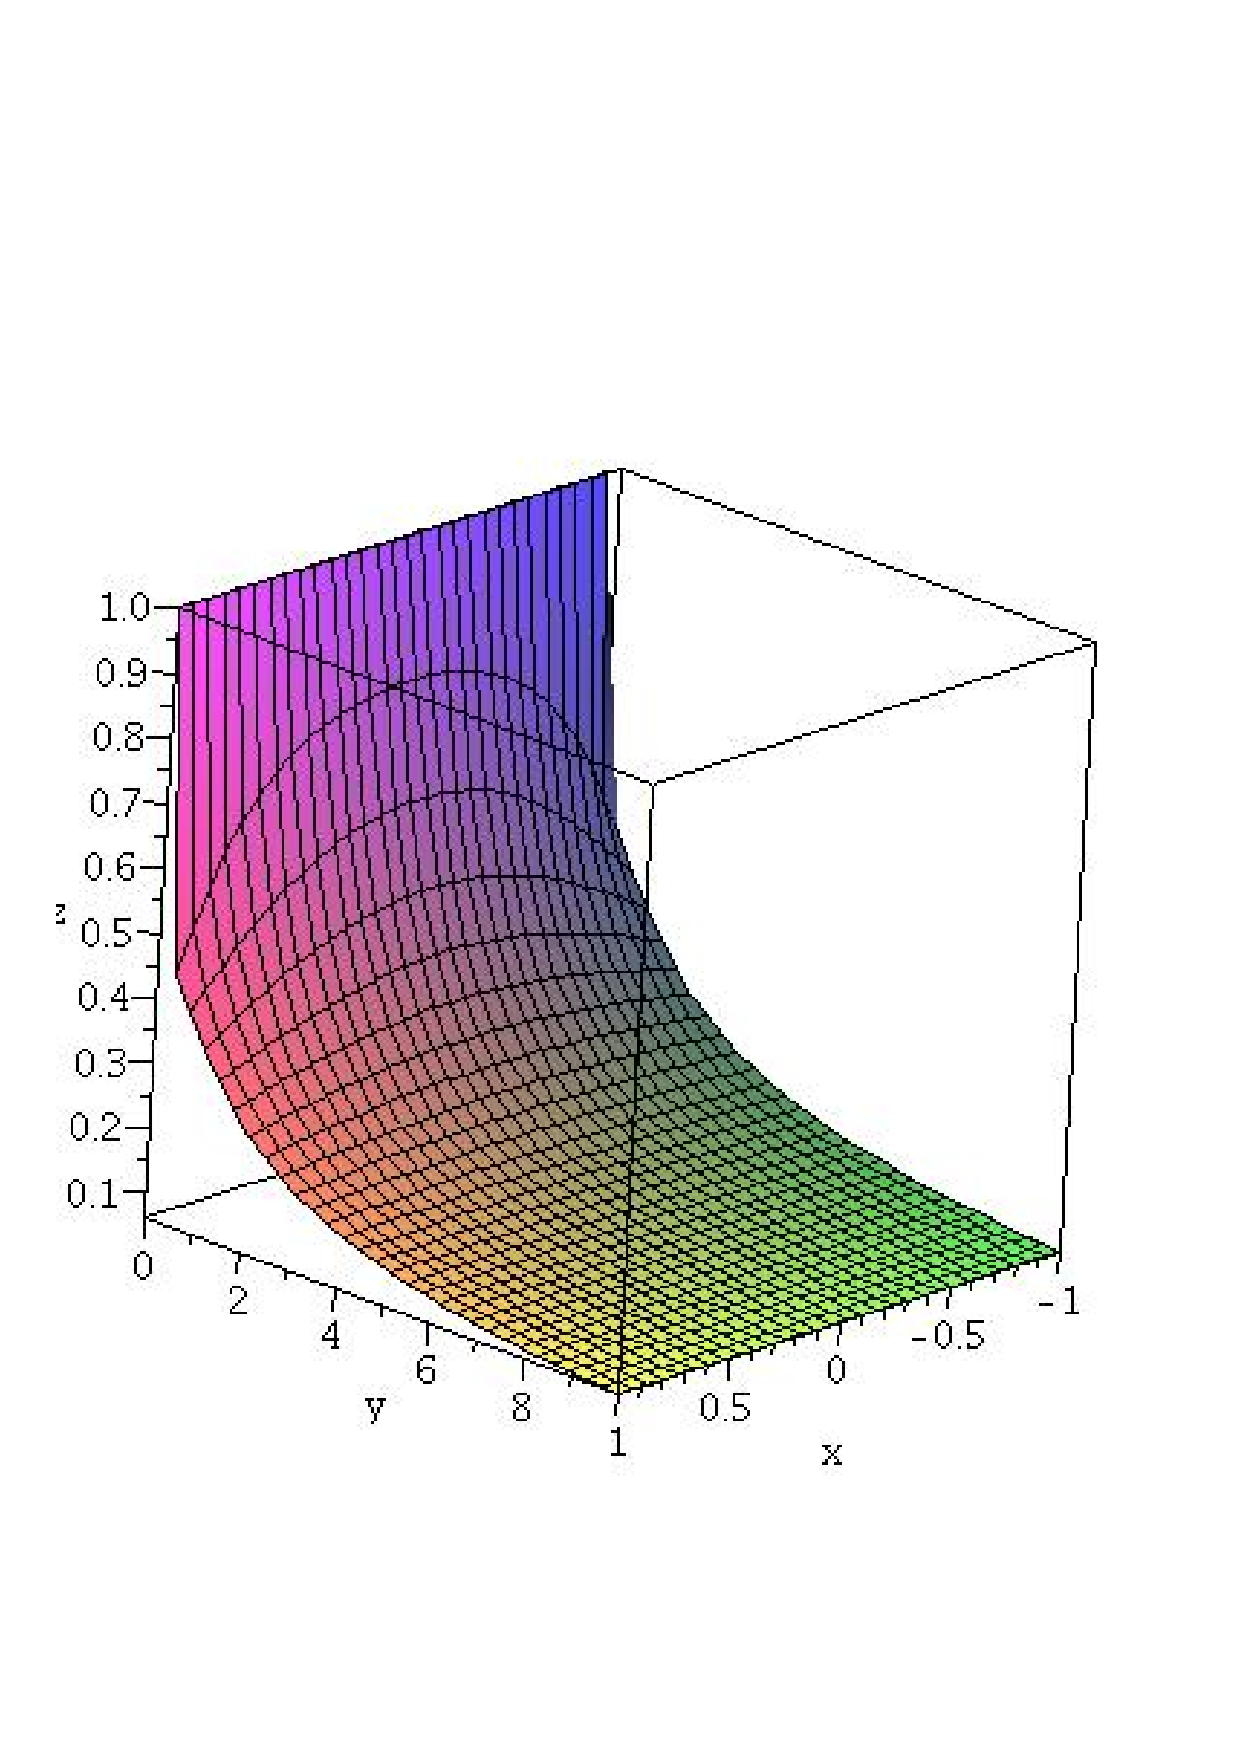
\includegraphics[width=100mm]{q2-plot.png}
        \caption{Plot of solution for exercise 2}
        \label{fig:q2-plot}
    \end{figure}

    \section*{Exercise 3}
    A PDE problem is given by
    \begin{gather*}
        \Delta u = 0,\quad (x,y)\in(0,\pi)^2, \\
        u(0,y)=0,\:\: u_x(\pi,y)+2u(\pi,y)=0,\\
        u(x,0)=0,\:\: u(x,\pi)=x(1-x)
    \end{gather*}
    The problem is solved using separation of variables. Therefore the solutions is given by
    \begin{equation*}
        u_n(x,y) = X_n(x)Y_n(y)
    \end{equation*}
    From $\Delta u=0$ we get
    \begin{align*}
        X_n''Y_n + X_nY_n'' &= 0 \myimp\\
        \frac{X_n''}{X_n} &= -\frac{Y_n''}{Y_n}
    \end{align*}
    and since the left side is independent of $y$ and the right side independent of $x$ we get
    \begin{align}\label{eq:sep}
        \frac{X_n''}{X_n} = -\frac{Y_n''}{Y_n} = -\lambda_n
    \end{align}
    Focusing on $X_n$ we get the ODE
    \begin{gather*}
        X_n'' + \lambda_n X_n = 0, \\
        X_n(0) = 0,\quad X_n'(\pi) + 2X_n(\pi) = 0
    \end{gather*}
    Now we are given that all eigenvalues $\lambda_n=\beta_n^2$ are positive. Then the solutions for the ODE of $X$ are
    \begin{equation*}
        X_n(x) = A_n\cos(\beta_n x) + B_n\sin(\beta_n x)
    \end{equation*}
    Using the first boundary condition gives
    \begin{align*}
        X_n(0) = A_n = 0
    \end{align*}
    The second boundary condition then gives
    \begin{align*}
        X_n'(\pi) + 2X_n(\pi) &= B_n\beta_n\cos(\beta_n \pi) + 2B_n\sin(\beta_n \pi) \\
        &= 0 \myimp \\
        \beta_n\cos(\beta_n\pi) &= -2\sin(\beta_n\pi) \\
        -\frac{\beta_n}{2} &= \tan(\beta_n\pi)
    \end{align*}
    The eigenvalues are given as solutions to this equation and the corresponding eigenfunctions are $\sin(\beta_n x)$. \par
    From (\ref{eq:sep}) and the boundary conditions of the original PDE the ODE for $Y_n$ is given by
    \begin{gather*}
        Y_n'' - \lambda Y_n = 0,\quad Y_n(0) = 0
    \end{gather*}
    This ODE has exponential solutions that for convenience are written
    \begin{equation*}
        Y_n(y) = C_n\cosh(\beta_n y) + D_n\sinh(\beta_n y)
    \end{equation*}
    From the homogeneous boundary condition we get
    \begin{equation*}
        Y_n(0) = C_n = 0
    \end{equation*}
    and we can then write the solution that satifies all the homogeneous boundary conditions for the PDE as
    \begin{equation*}
        u(x,y) = \sum_{n=0}^\infty D_n\sinh(\beta_n y)\sin(\beta_n x)
    \end{equation*}
    To determine the coefficients $D_n$ we use the inhomogeneous boundary condition
    \begin{align*}
        u(x,\pi) = \sum_{n=0}^\infty D_n\sinh(\beta_n \pi)\sin(\beta_n x) = x(1-x)
    \end{align*}
    This is the Fourier sine series for the function $\phi(x)=x(1-x)$ and from equation 5.1.4 we find the coefficients $D_n$ by
    \begin{equation*}
        D_n = \frac{2}{\pi\sinh(\beta_n\pi)}\int_0^\pi x(1-x)\sin(\beta_n x)\,dx
    \end{equation*}
\end{document}
